% To make a PDF from this source, use the pdflatex command.
\documentclass[helvetica,english,utf8,notitle,nologo]{beamer}
\usetheme{default}
\usecolortheme{seahorse}
\usepackage{graphicx}
\graphicspath{ {images/} }

\begin{document}

\title{Intro to Ruby Programming}
\author{Carlos Konstanski}

\frame{\titlepage}

\begin{frame}
  \frametitle{Presentation Materials Available Online At:}
  \href{url}{https://github.com/ckonstanski/ruby-presentation}
\end{frame}

\begin{frame}
  \frametitle{Supported Platforms}

  Ruby runs on Linux, Mac OSX and Windows. A hugely popular
  configuration is Mac OSX for the development workstation and Linux
  for the server.

  This presentation is done entirely on Linux. Things should work very
  similarly on Mac OSX. I will not address Windows at all because I
  have no familiarity with it nor a means to test with it.

\end{frame}

\begin{frame}
  \frametitle{Ruby Is Interpreted}

  Ruby is an interpreted language. There is no visible compilation
  step where your source code is transformed into bytecode or machine
  code. Of course the characters you type in your source files need to
  be converted to something that is easier for the machine to execute,
  but it is retained only in memory and never written to an object
  file.

  Ruby is implemented in C. The ruby interpreter is called the Matz
  Ruby Interpreter (MRI). It is named after the creator of ruby,
  Yukihiro Matsumoto (aka "Matz").

  Ruby's execution speed is faster than perl, PHP and python, but
  slower than byte-compiled python. All of these languages are an
  order of magnitude slower than classic compiled languages like Java,
  C\# and Common Lisp. These in turn are about 3-6 times slower than
  C.
\end{frame}

\begin{frame}
  \frametitle{Where is Ruby Used?}

  Standalone ruby applications:

  \begin{itemize}
  \item Puppet
  \item Chef
  \item Metasploit
  \item Vagrant
  \end{itemize}

  Ruby websites:

  \begin{itemize}
  \item Twitter (started with ruby; now uses something else)
  \item Groupon
  \item Bloomberg
  \item AirBnB
  \item Hulu
  \item Github
  \end{itemize}
\end{frame}

\begin{frame}
  \frametitle{Ruby Has a Version Explosion Issue}

  There is an unfortunate proliferation of ruby versions. Some
  non-backward-compatible changes between versions resulted in an
  inability to retire old versions. I'm not sure that the problem
  still exists with recent versions, but the die has been cast. Right
  now I have four versions of ruby installed on my laptop.

  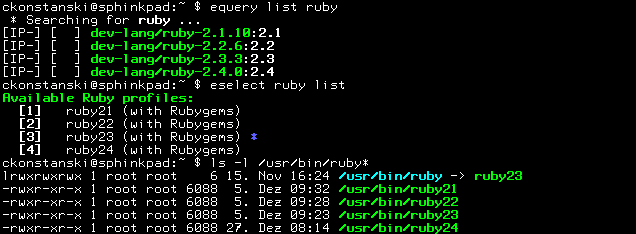
\includegraphics[scale=0.5]{eselect_1}
\end{frame}

\begin{frame}
  \frametitle{Ruby Version Management}

  There are systems similar to python's virtualenv that help manage
  the version problem by installing copies of ruby and libraries that
  are local to an application.

  \begin{itemize}
  \item rvm
  \item rbenv
  \item ruby-build
  \item chruby
  \item ruby-install
  \end{itemize}

  If you don't need to manage the ruby interpreter itself, but only
  need to manage the libraries on a per-application basis:

  \begin{itemize}
  \item rubygems
  \item bundler
  \end{itemize}
\end{frame}

\begin{frame}
  \frametitle{Running Ruby}
  \begin{itemize}
  \item Interactively via IRB
  \item Source code stored in files
  \end{itemize}
\end{frame}

\begin{frame}
  \frametitle{IRB}

  IRB is the interactive ruby shell. You can type ad-hoc ruby
  statements at the IRB prompt and they will execute immediately. It
  is a great tool for iterative programming and for testing out new
  ideas.

  Here is a very simple example of an IRB session:

  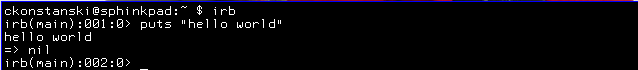
\includegraphics[scale=0.5]{irb_1}

  And here is a slightly more involved example which demonstrates that
  the environment saves the state of objects that you create via the
  statements that you execute (until you exit):

  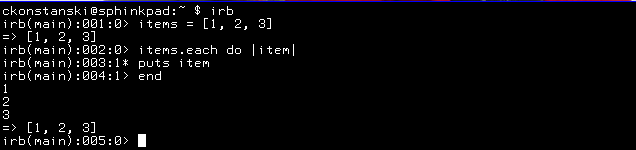
\includegraphics[scale=0.5]{irb_2}

  Type exit, quit or CTRL-d to exit an IRB session.
\end{frame}

\begin{frame}
  \frametitle{Source Files}

  Like all programming languages, you can create source files that
  contain the statements you wish to run. Ruby source files generally
  have an .rb extension.

  Two ways to launch a script:
  \begin{itemize}
  \item Shebang
    \begin{itemize}
    \item Requires executable permissions
    \item Uses the interpreter specified in the shebang
    \item Can be treated like any executable
    \end{itemize}
  \item ruby [filename]
    \begin{itemize}
    \item Requires no executable permissions
    \item Can choose which ruby interpreter to use (if you have
      multiple)
    \item Overrides the shebang
    \end{itemize}
  \end{itemize}
\end{frame}

\begin{frame}
  \frametitle{Ruby Syntax}
  \begin{itemize}
  \item A C-style language (English-like)
  \item Statements terminated by semicolon or newline
    \begin{itemize}
    \item Semicolons are rare
    \item Mostly used to put multiple statements on one line
    \item In an IRB session a semicolon-terminated statement will not
      ``commit''. It will wait until a newline-terminated statement is
      entered.
    \end{itemize}
  \item Code blocks are delimited with curly braces or end
    keywords
     \begin{itemize}
     \item Curly braces are only used in closures
     \item begin...end blocks are also used in closures, as well as if
       statements, while loops, etc.
     \item In several cases begin is replaced by do
       \begin{itemize}
       \item loop
       \item closures
       \end{itemize}
     \end{itemize}
     \item The ruby equivalent of try...catch...finally is
       begin...rescue...ensure...end
  \end{itemize}
\end{frame}

\begin{frame}
  \frametitle{Ruby Syntax: Boolean operators}

  Ruby supports ``both'' types of boolean operators.

  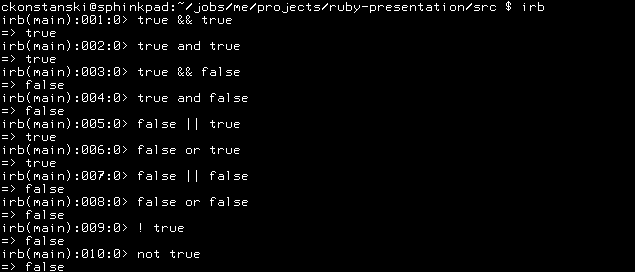
\includegraphics[scale=0.5]{irb_5}
\end{frame}

\begin{frame}
  \frametitle{Ruby Syntax: while-loop}

  A while-loop with conditional at end:

  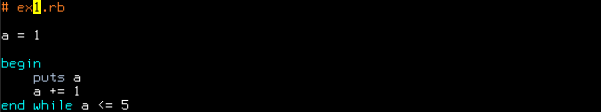
\includegraphics[scale=0.53]{src_1}

  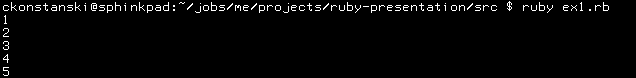
\includegraphics[scale=0.5]{out_1}

  A while-loop with conditional at beginning:

  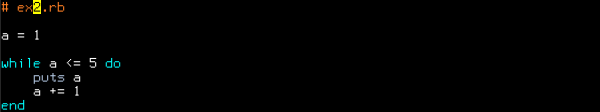
\includegraphics[scale=0.53]{src_2}

  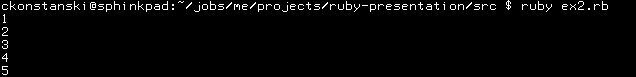
\includegraphics[scale=0.5]{out_2}
\end{frame}

\begin{frame}
  \frametitle{Ruby Syntax: while-loop, if-statement}

  A while-loop on one line (and a glimpse at ``functional'' operations):

  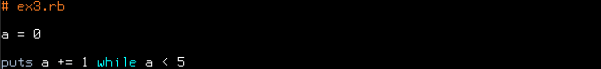
\includegraphics[scale=0.53]{src_3}

  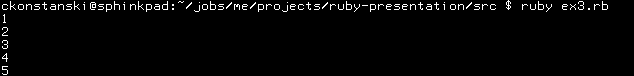
\includegraphics[scale=0.5]{out_3}

  if-statements in a block and on one line:

  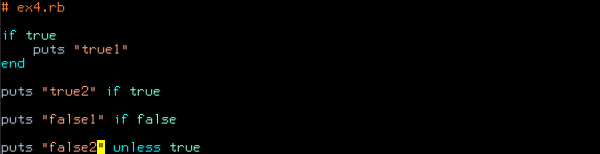
\includegraphics[scale=0.53]{src_4}

  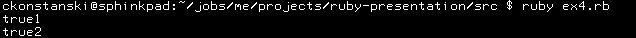
\includegraphics[scale=0.5]{out_4}
\end{frame}

\begin{frame}
  \frametitle{Ruby Syntax: Collection Types}

  Ruby has built-in support for arrays and hashes.

  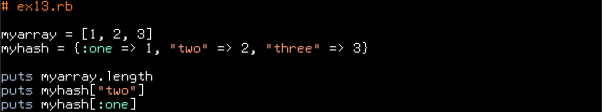
\includegraphics[scale=0.53]{src_13}

  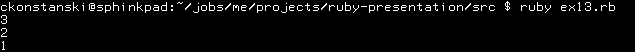
\includegraphics[scale=0.5]{out_13}
\end{frame}

\begin{frame}
  \frametitle{Ruby Syntax: Functions, Print Formatting}

  Functions always return something even if it's nil. The return value
  is the last value to be computed in the function body. The return
  keyword is unnecessary.

  When printing a computed value embedded in a string literal, ruby
  uses a syntax reminiscent of BASH, PHP or perl.

  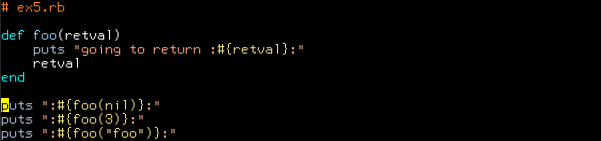
\includegraphics[scale=0.53]{src_5}

  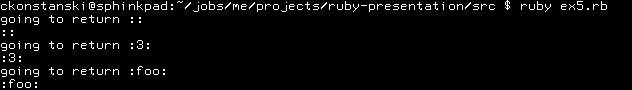
\includegraphics[scale=0.5]{out_5}
\end{frame}

\begin{frame}
  \frametitle{Ruby Syntax: Symbols}

  Ruby symbols are very simple objects: they are just names. They can
  be used to name certain things in place of a string name. The
  advantage: symbols are globally unique. While there can exist two
  separate strings that are equivalent, any attempt to create a second
  instance of a symbol with a particular name simply returns the
  already-existing symbol. Therefore symbols are more space-efficient
  and comparing symbols is faster. Comparing two symbols is simply a
  comparison of their IDs.

  You can use a symbol in place of a string as long as the value never
  needs to change (since symbols are immutable) and you don't need any
  of the methods of the String class. The most common usage is for the
  keys of a hash.
\end{frame}

\begin{frame}
  \frametitle{Ruby Syntax: Keyword Arguments}

  Functions can have named arguments that have default values.

  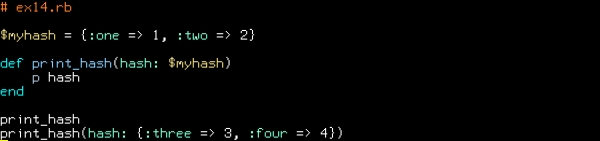
\includegraphics[scale=0.53]{src_14}

  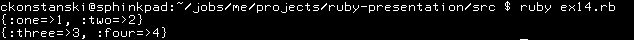
\includegraphics[scale=0.5]{out_14}
\end{frame}

\begin{frame}
  \frametitle{Ruby Syntax: nil, true, false}

  Ruby has three special objects to represent the values of nil, true
  and false: NilClass, TrueClass and FalseClass respectively. The
  keywords nil, true and false are used to refer to these special
  objects.

  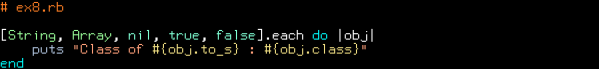
\includegraphics[scale=0.53]{src_8}

  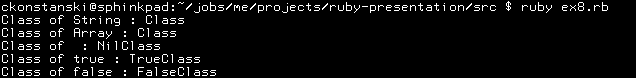
\includegraphics[scale=0.5]{out_8}
\end{frame}

\begin{frame}
  \frametitle{Ruby Syntax: Subshell}

  Ruby is a good choice for shell scripting because, like perl and
  BASH, it lets you execute shell commands by enclosing them in
  backquotes. The result of the subshell is a string that contains the
  STDOUT of the command that was run in the subshell.

  Another thing that ruby shares in common with perl is its regular
  expression syntax.
  
  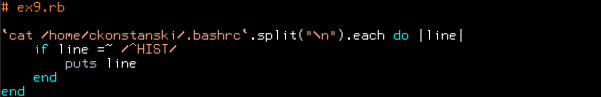
\includegraphics[scale=0.53]{src_9}

  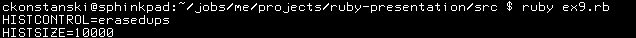
\includegraphics[scale=0.5]{out_9}
\end{frame}

\begin{frame}
  \frametitle{Ruby Syntax: Splat}

  Ruby has an array structuring/destructuring operator: the splat. It
  is most often used to group or degroup function arguments.

  Example of function argument structuring:

  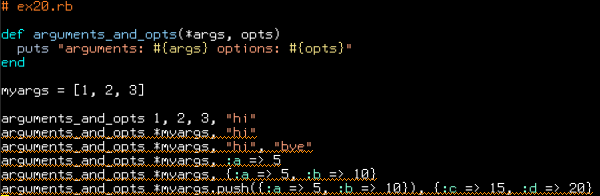
\includegraphics[scale=0.53]{src_20}

  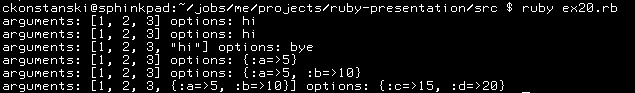
\includegraphics[scale=0.5]{out_20}
\end{frame}

\begin{frame}
  \frametitle{Ruby Syntax: Splat}

  Example of function argument destructuring:

  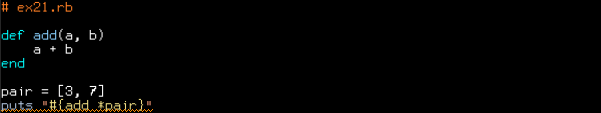
\includegraphics[scale=0.53]{src_21}

  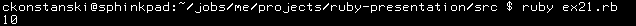
\includegraphics[scale=0.5]{out_21}
\end{frame}

\begin{frame}
  \frametitle{Including Files}

  Ruby supports file includes. To include a file that is in the
  include path, use ``require''. To include a file anywhere on the
  filesystem, use ``require\_relative''.

  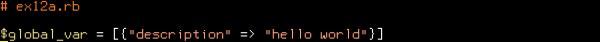
\includegraphics[scale=0.53]{src_12a}

  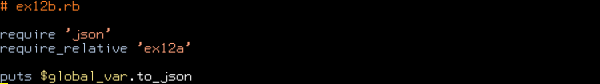
\includegraphics[scale=0.53]{src_12b}

  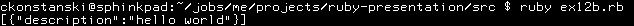
\includegraphics[scale=0.5]{out_12}
\end{frame}

\begin{frame}
  \frametitle{Ruby Is Object-Oriented}

  Everything is an object, even strings and numbers:

  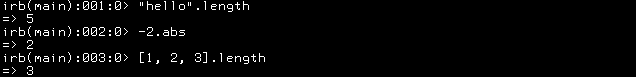
\includegraphics[scale=0.5]{irb_3}

  Any object, even the built-in ones, can be extended at runtime. This
  example shows the built-in Array object being extended with a new
  method:

  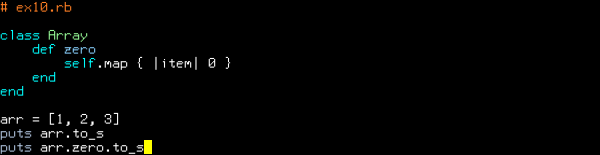
\includegraphics[scale=0.53]{src_10}
  
  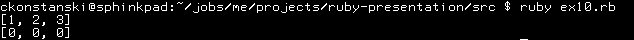
\includegraphics[scale=0.5]{out_10}

  This technique is called metaprogramming.
\end{frame}

\begin{frame}
  \frametitle{Classes}

  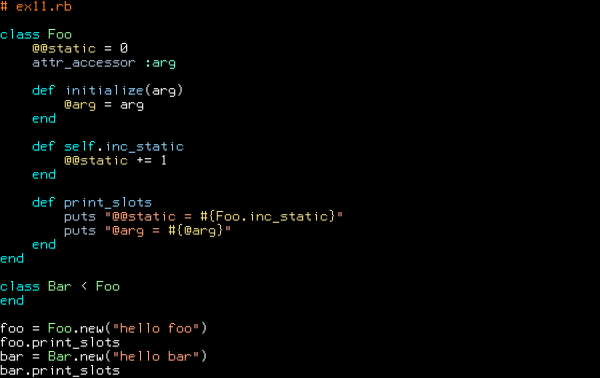
\includegraphics[scale=0.53]{src_11}
  
  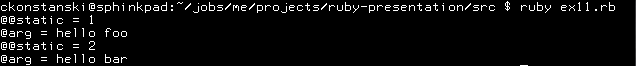
\includegraphics[scale=0.5]{out_11}
\end{frame}

\begin{frame}
  \frametitle{Error Handling}

  Unhandled errors:

  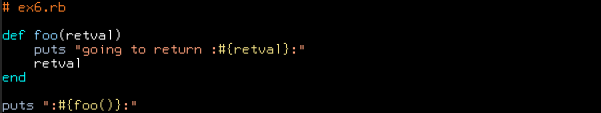
\includegraphics[scale=0.53]{src_6}

  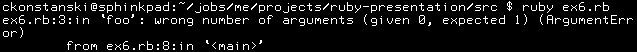
\includegraphics[scale=0.5]{out_6}

  The classic nil:NilClass (NoMethodError):

  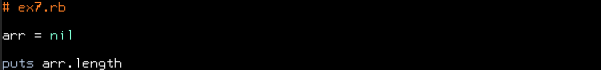
\includegraphics[scale=0.53]{src_7}

  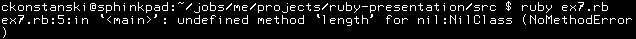
\includegraphics[scale=0.5]{out_7}
\end{frame}

\begin{frame}
  \frametitle{Error Handling}

  Catching and handling errors:

  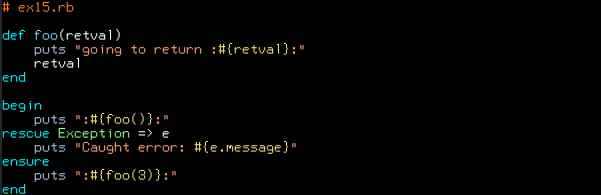
\includegraphics[scale=0.53]{src_15}

  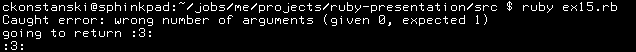
\includegraphics[scale=0.5]{out_15}
\end{frame}

\begin{frame}
  \frametitle{Closures}

  A ruby closure is the most foreign-looking syntactical construct you
  will encounter. We've seen this concept in action already when we
  iterated over arrays with each().

  A closure is really a method call. The method contains a yield
  statement. 
\end{frame}

\begin{frame}
  \frametitle{Closures}

  Here is an example lifted directly from stackoverflow:

  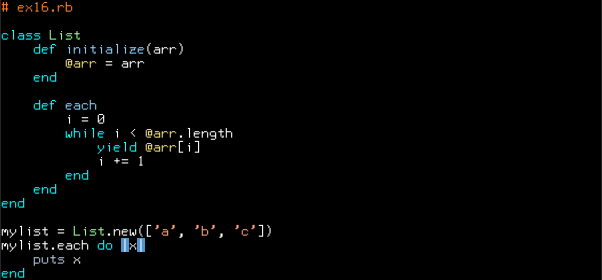
\includegraphics[scale=0.53]{src_16}

  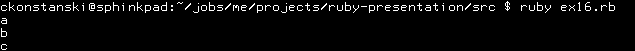
\includegraphics[scale=0.5]{out_16}

  In this example, ``x'' is the iterator and ``puts x'' is the body of
  the closure.
\end{frame}

\begin{frame}
  \frametitle{Closures}

  There is a better name for the code that comprises the closure
  body. It's called a lambda function. A lambda function is a function
  with no name. Sometimes it's called an anonymous function.

  There are actually to ways to enclose the lambda function: in a
  do...end block or in curly braces. They both function the same. I
  can find no other reason than stylistic preference to choose one
  over the other. It is common for single-line invocations to use
  curly braces. For this purpose a do...end block is not feasible
  unless you resort to using semicolons to terminate statements.

  A method containing a yield statement can be thought to have an
  extra invisible argument: the lambda function of the calling
  closure. Each time the yield statement is encountered, it runs the
  lambda function feeding in the current iterator value(s) as
  arguments. Lambda functions have arguments just like any other
  function. The argument(s) are the variables that appear inside the
  pipes.
\end{frame}

\begin{frame}
  \frametitle{Closures}

  A simple example of a closure that has more than one iterator
  variable, or lambda argument if you will:

  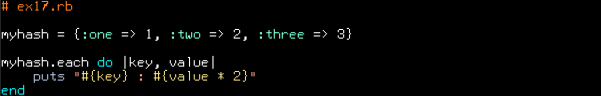
\includegraphics[scale=0.53]{src_17}

  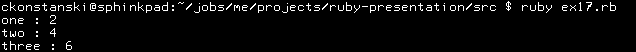
\includegraphics[scale=0.5]{out_17}
\end{frame}

\begin{frame}
  \frametitle{Closures}

  The entire closure can be treated as an object. It can be followed
  by the dot operator and a method call. The real object is the return
  value of the closure. Such an invocation requires that the closure
  actually returns something (other than nil).

  The return value of an Array.each() call is different than that of
  an Array.map() call. We saw how to use map() to transform each
  element of an array. What if we did the same thing but used each()
  instead? The values returned by each iteration of the lambda
  function don't get saved anywhere. The return value of the closure
  is an array consisting of the original values in the array.
  
  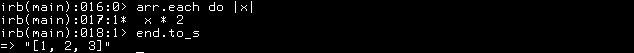
\includegraphics[scale=0.5]{irb_7}

  If you just want to do do work with each element of an array but
  don't care about collecting the results, use each(). If you want to
  create a new array that is the result of transforming each value of
  the original array, use map().
\end{frame}

\begin{frame}
  \frametitle{Closures}

  Closures are used for a lot more than iterating over
  arrays. Iteration is just the most obvious and oft-used
  example. This paradigm of feeding a lambda function into a method
  and calling yield on it has other uses as well.
\end{frame}

\begin{frame}
  \frametitle{Closures}

  A very simple example of a closure:

  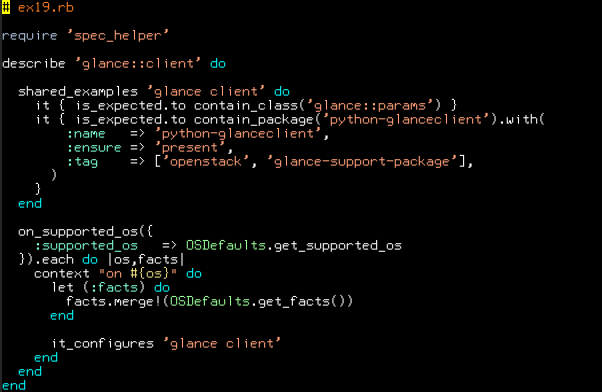
\includegraphics[scale=0.53]{src_19}

  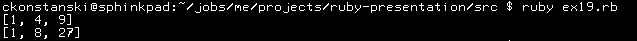
\includegraphics[scale=0.5]{out_19}
\end{frame}

\begin{frame}
  \frametitle{Closures}

  The same thing implemented as a metaprogrammed new method on the
  Array class:

  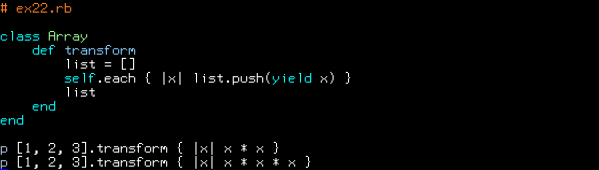
\includegraphics[scale=0.53]{src_22}

  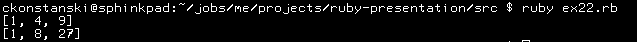
\includegraphics[scale=0.5]{out_22}
\end{frame}

\begin{frame}
  \frametitle{Closures}

  Chef is an enterprise configuration management platform. It is
  implemented entirely in ruby. The configuration you write is also
  ruby. It is a DSL (Domain Specific Language) that is full of
  closures. Here is a short example of a chef recipe file:

  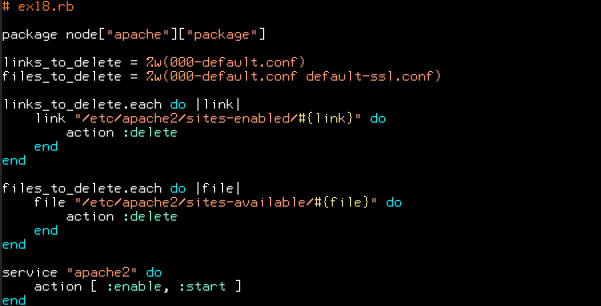
\includegraphics[scale=0.53]{src_18}
\end{frame}

\begin{frame}
  \frametitle{Multithreading}

  Ruby has a simple but effective threading API. See the docs for the
  full feature set. Here we will look at a simple example that
  includes a mutex.

  An interesting thing happened when I ran the example. When ran
  repeatedly, sometimes the second thread actually started first, or
  at least it gained the lock first. This shows that you cannot depend
  on threads and mutexes running in any sort of order.
\end{frame}

\begin{frame}
  \frametitle{Multithreading}

  \includegraphics[scale=0.53]{src_23}

  \includegraphics[scale=0.5]{out_23}
\end{frame}

\end{document}
